\documentclass[12pt,letterpaper]{hmcpset}
\usepackage[margin=1in]{geometry}
\usepackage{graphicx}
\usepackage{amsmath,amssymb}
\usepackage{enumerate}
\usepackage{hyperref}
\usepackage{parskip}

% Theorems
\usepackage{amsthm}
\renewcommand\qedsymbol{$\blacksquare$}
\makeatletter
\@ifclassloaded{article}{
    \newtheorem{definition}{Definition}[section]
    \newtheorem{example}{Example}[section]
    \newtheorem{theorem}{Theorem}[section]
    \newtheorem{corollary}{Corollary}[theorem]
    \newtheorem{lemma}{Lemma}[theorem]
}{
}
\makeatother

% Random Stuff
\setlength\unitlength{1mm}

\newcommand{\insertfig}[3]{
\begin{figure}[htbp]\begin{center}\begin{picture}(120,90)
\put(0,-5){\includegraphics[width=12cm,height=9cm,clip=]{#1.eps}}\end{picture}\end{center}
\caption{#2}\label{#3}\end{figure}}

\newcommand{\insertxfig}[4]{
\begin{figure}[htbp]
\begin{center}
\leavevmode \centerline{\resizebox{#4\textwidth}{!}{\input
#1.pstex_t}}
\caption{#2} \label{#3}
\end{center}
\end{figure}}

\long\def\comment#1{}

\newcommand\norm[1]{\left\lVert#1\right\rVert}
\DeclareMathOperator*{\argmin}{arg\,min}
\DeclareMathOperator*{\argmax}{arg\,max}

% bb font symbols
\newfont{\bbb}{msbm10 scaled 700}
\newcommand{\CCC}{\mbox{\bbb C}}

\newfont{\bbf}{msbm10 scaled 1100}
\newcommand{\CC}{\mbox{\bbf C}}
\newcommand{\PP}{\mbox{\bbf P}}
\newcommand{\RR}{\mbox{\bbf R}}
\newcommand{\QQ}{\mbox{\bbf Q}}
\newcommand{\ZZ}{\mbox{\bbf Z}}
\renewcommand{\SS}{\mbox{\bbf S}}
\newcommand{\FF}{\mbox{\bbf F}}
\newcommand{\GG}{\mbox{\bbf G}}
\newcommand{\EE}{\mbox{\bbf E}}
\newcommand{\NN}{\mbox{\bbf N}}
\newcommand{\KK}{\mbox{\bbf K}}
\newcommand{\KL}{\mbox{\bbf KL}}

% Vectors
\renewcommand{\aa}{{\bf a}}
\newcommand{\bb}{{\bf b}}
\newcommand{\cc}{{\bf c}}
\newcommand{\dd}{{\bf d}}
\newcommand{\ee}{{\bf e}}
\newcommand{\ff}{{\bf f}}
\renewcommand{\gg}{{\bf g}}
\newcommand{\hh}{{\bf h}}
\newcommand{\ii}{{\bf i}}
\newcommand{\jj}{{\bf j}}
\newcommand{\kk}{{\bf k}}
\renewcommand{\ll}{{\bf l}}
\newcommand{\mm}{{\bf m}}
\newcommand{\nn}{{\bf n}}
\newcommand{\oo}{{\bf o}}
\newcommand{\pp}{{\bf p}}
\newcommand{\qq}{{\bf q}}
\newcommand{\rr}{{\bf r}}
\renewcommand{\ss}{{\bf s}}
\renewcommand{\tt}{{\bf t}}
\newcommand{\uu}{{\bf u}}
\newcommand{\ww}{{\bf w}}
\newcommand{\vv}{{\bf v}}
\newcommand{\xx}{{\bf x}}
\newcommand{\yy}{{\bf y}}
\newcommand{\zz}{{\bf z}}
\newcommand{\0}{{\bf 0}}
\newcommand{\1}{{\bf 1}}

% Matrices
\newcommand{\Ab}{{\bf A}}
\newcommand{\Bb}{{\bf B}}
\newcommand{\Cb}{{\bf C}}
\newcommand{\Db}{{\bf D}}
\newcommand{\Eb}{{\bf E}}
\newcommand{\Fb}{{\bf F}}
\newcommand{\Gb}{{\bf G}}
\newcommand{\Hb}{{\bf H}}
\newcommand{\Ib}{{\bf I}}
\newcommand{\Jb}{{\bf J}}
\newcommand{\Kb}{{\bf K}}
\newcommand{\Lb}{{\bf L}}
\newcommand{\Mb}{{\bf M}}
\newcommand{\Nb}{{\bf N}}
\newcommand{\Ob}{{\bf O}}
\newcommand{\Pb}{{\bf P}}
\newcommand{\Qb}{{\bf Q}}
\newcommand{\Rb}{{\bf R}}
\newcommand{\Sb}{{\bf S}}
\newcommand{\Tb}{{\bf T}}
\newcommand{\Ub}{{\bf U}}
\newcommand{\Wb}{{\bf W}}
\newcommand{\Vb}{{\bf V}}
\newcommand{\Xb}{{\bf X}}
\newcommand{\Yb}{{\bf Y}}
\newcommand{\Zb}{{\bf Z}}

% Calligraphic
\newcommand{\Ac}{{\cal A}}
\newcommand{\Bc}{{\cal B}}
\newcommand{\Cc}{{\cal C}}
\newcommand{\Dc}{{\cal D}}
\newcommand{\Ec}{{\cal E}}
\newcommand{\Fc}{{\cal F}}
\newcommand{\Gc}{{\cal G}}
\newcommand{\Hc}{{\cal H}}
\newcommand{\Ic}{{\cal I}}
\newcommand{\Jc}{{\cal J}}
\newcommand{\Kc}{{\cal K}}
\newcommand{\Lc}{{\cal L}}
\newcommand{\Mc}{{\cal M}}
\newcommand{\Nc}{{\cal N}}
\newcommand{\Oc}{{\cal O}}
\newcommand{\Pc}{{\cal P}}
\newcommand{\Qc}{{\cal Q}}
\newcommand{\Rc}{{\cal R}}
\newcommand{\Sc}{{\cal S}}
\newcommand{\Tc}{{\cal T}}
\newcommand{\Uc}{{\cal U}}
\newcommand{\Wc}{{\cal W}}
\newcommand{\Vc}{{\cal V}}
\newcommand{\Xc}{{\cal X}}
\newcommand{\Yc}{{\cal Y}}
\newcommand{\Zc}{{\cal Z}}

% Bold greek letters
\newcommand{\alphab}{\hbox{\boldmath$\alpha$}}
\newcommand{\betab}{\hbox{\boldmath$\beta$}}
\newcommand{\gammab}{\hbox{\boldmath$\gamma$}}
\newcommand{\deltab}{\hbox{\boldmath$\delta$}}
\newcommand{\etab}{\hbox{\boldmath$\eta$}}
\newcommand{\lambdab}{\hbox{\boldmath$\lambda$}}
\newcommand{\epsilonb}{\hbox{\boldmath$\epsilon$}}
\newcommand{\nub}{\hbox{\boldmath$\nu$}}
\newcommand{\mub}{\hbox{\boldmath$\mu$}}
\newcommand{\zetab}{\hbox{\boldmath$\zeta$}}
\newcommand{\phib}{\hbox{\boldmath$\phi$}}
\newcommand{\psib}{\hbox{\boldmath$\psi$}}
\newcommand{\thetab}{\hbox{\boldmath$\theta$}}
\newcommand{\taub}{\hbox{\boldmath$\tau$}}
\newcommand{\omegab}{\hbox{\boldmath$\omega$}}
\newcommand{\xib}{\hbox{\boldmath$\xi$}}
\newcommand{\sigmab}{\hbox{\boldmath$\sigma$}}
\newcommand{\pib}{\hbox{\boldmath$\pi$}}
\newcommand{\rhob}{\hbox{\boldmath$\rho$}}

\newcommand{\Gammab}{\hbox{\boldmath$\Gamma$}}
\newcommand{\Lambdab}{\hbox{\boldmath$\Lambda$}}
\newcommand{\Deltab}{\hbox{\boldmath$\Delta$}}
\newcommand{\Sigmab}{\hbox{\boldmath$\Sigma$}}
\newcommand{\Phib}{\hbox{\boldmath$\Phi$}}
\newcommand{\Pib}{\hbox{\boldmath$\Pi$}}
\newcommand{\Psib}{\hbox{\boldmath$\Psi$}}
\newcommand{\Thetab}{\hbox{\boldmath$\Theta$}}
\newcommand{\Omegab}{\hbox{\boldmath$\Omega$}}
\newcommand{\Xib}{\hbox{\boldmath$\Xi$}}

% mixed symbols
\newcommand{\sinc}{{\hbox{sinc}}}
\newcommand{\diag}{{\hbox{diag}}}
\renewcommand{\det}{{\hbox{det}}}
\newcommand{\trace}{{\hbox{tr}}}
\newcommand{\tr}{\trace}
\newcommand{\sign}{{\hbox{sign}}}
\renewcommand{\arg}{{\hbox{arg}}}
\newcommand{\var}{{\hbox{var}}}
\newcommand{\cov}{{\hbox{cov}}}
\renewcommand{\Re}{{\rm Re}}
\renewcommand{\Im}{{\rm Im}}
\newcommand{\eqdef}{\stackrel{\Delta}{=}}
\newcommand{\defines}{{\,\,\stackrel{\scriptscriptstyle \bigtriangleup}{=}\,\,}}
\newcommand{\<}{\left\langle}
\renewcommand{\>}{\right\rangle}
\newcommand{\Psf}{{\sf P}}
\newcommand{\T}{\top}
\newcommand{\m}[1]{\begin{bmatrix} #1 \end{bmatrix}}

% info for header block in upper right hand corner
\name{}
\class{Math189R SP19}
\assignment{Homework 2}
\duedate{Monday, Feb 11, 2019}

\begin{document}

Feel free to work with other students, but make sure you write up the homework
and code on your own (no copying homework \textit{or} code; no pair programming).
Feel free to ask students or instructors for help debugging code or whatever else,
though.
\newline
\newline
The starter files can be found under the Resource tab on course website. The graphs for problem 3 generated by the sample solution could be found in the corresponding zipfile. These graphs only serve as references to your implementation. You should generate your own graphs for submission. Please print out all the graphs generated by your own code and submit them together with the written part, and make sure you upload the code to your Github repository.\\

\begin{problem}[1]
	(\textbf{Murphy 8.3}) Gradient and Hessian of the log-likelihood for
	logistic regression.
	\begin{enumerate}[(a)]
		\item Let $\sigma(x) = \frac{1}{1 + e^{-x}}$ be the sigmoid function. Show that
		$$
		\sigma'(x) = \sigma(x)\left[1 - \sigma(x)\right].
		$$
		\item Using the previous result and the chain rule of calculus, derive an
		expression for the gradient of the log likelihood for logistic regression.
		\item The Hessian can be written as $\Hb=\Xb^\T\Sb\Xb$ where $\Sb =
		\diag(\mu_1(1-\mu_1), \dots, \mu_n(1-\mu_n))$. Derive this and show that
		$\Hb \succeq 0$ ($A \succeq 0$ means that $A$ is positive semidefinite).\\
	\end{enumerate} 

\textit{Hint:} Use the \textbf{negative} log-likelihood of logistic regression for this problem.
\end{problem}
\begin{solution}
	Part a: Given $\sigma(x) = \frac{1}{1 + e^{-x}}$, we can find $\sigma'(x)$ as the following.
	
	\begin{align*}
		\sigma'(x) &= \frac{d}{dx}(\sigma(x))\\
		&= \frac{d}{dx}(\frac{1}{1+e^{-x}})\\
		&= e^{-x}(1+e^{-x})^{-2}\\
		&=  \frac{1}{1 + e^{-x}} \cdot  \frac{e^{-x}}{1 + e^{-x}}\\
		&= \frac{1}{1 + e^{-x}} \cdot  \frac{1 + e^{-x} - 1}{1 + e^{-x}}\\
		&= \frac{1}{1 + e^{-x}} \cdot  (1- \frac{1}{1 + e^{-x}})\\
		&= \sigma(x)[1-\sigma(x)]\\	
	\end{align*}

	Part b:
	By definition, the negative log likelihood for logistic regression is the following
	$$nll(\theta) = - \sum_{i} y_i \log(\sigma(\theta^T x_i)) + (1 - y_i)\log(1 - \sigma(\theta^T x_i))$$

Next, we can find the gradient of $nll$ with respect to $\theta$.
\begin{align*}
	\nabla_{\theta}nll(\theta) &= - \sum_{i} \frac{y_i}{\sigma(\theta^T x_i)} \cdot \sigma'(\theta^T x_i) - \frac{(1 - y_i)}{1 - \sigma(\theta^T x_i)} \cdot -\sigma'(\theta^T x_i)\\
	&= - \sum_{i} y_i (1 - \sigma(\theta^T x_i)) - (1 - y_i)\sigma(\theta^T x_i)x_i\\
	&= - \sum_{i} y_i x_i - y_i \sigma(\theta^T x_i) x_i - \sigma(\theta^T x_i) x_i + y_i \sigma(\theta^T x_i) x_i\\
	&= \sum_{i} (\sigma(\theta^T x_i) - y_i) x_i\\
	&= \sum_{i} (\mu_i - y_i) x_i\\
	&= X^T (\mu - y)
\end{align*}


where $\mu_i = \sigma(\theta^T x_i)$ and $x_i$ is the $i^{th}$ column of $X^T$.

Part c: From part b, we have $nll(\theta))^T = \nabla_{\theta}[X^T (\mu - y)]^T$. Then, we can use this to find the Hessian matrix as the following.
\begin{align*}
H_{\theta} &= \nabla_{\theta} (\nabla_{\theta}nll(\theta))^T\\
& = \nabla_{\theta}[X^T (\mu - y)]^T\\
&= \nabla_{\theta} (\mu^T X - y^T X)\\
&= \nabla_{\theta} \mu^T X = \nabla_{\theta} \sigma(X\theta)^T X\\
&= X^T \text{diag}(\mu(1 - \mu))X\\
&= X^T SX
\end{align*}


where $ S = \text{diag}(\mu_1(1 - \mu_1),\ldots,\mu_n(1 - \mu_n)) $.

Note that since $S$ is a diagonal matrix, its eigenvalues are its diagonal entries, and it is positive semi-definite if the diagonal entries are greater than 0. Also note that $0 < \sigma(x) < 1$ for any $x$. Since $\mu_i = \sigma(\theta^T x_i)$, we can see that $\mu_i(1 - \mu_i) = \sigma(\theta^T x_i)(1 - \sigma(\theta^T x_i)) \geq 0$. Thus, $S$ is positive semi-definite. Thus, $H_\theta$ must also be semi-definite.

\end{solution}
\newpage

\begin{problem}[2]
	(\textbf{Murphy 2.11})
	Derive the normalization constant ($Z$) for a one dimensional
	zero-mean Gaussian
	$$
	\PP(x; \sigma^2) = \frac{1}{Z}\exp\left(-\frac{x^2}{2\sigma^2}\right)
	$$
	such that $\PP(x; \sigma^2)$ becomes a valid density.
\end{problem}
\begin{solution}
	By definition, a valid density function must integrate to one.
$$
\int_{\mathbb{R}} p(x;\sigma^2)dx = \int_{\mathbb{R}} \frac{1}{Z} \exp \left(-\frac{x^2}{2\sigma^2}\right) dx = \frac{1}{Z} \int_{\mathbb{R}} \exp \left(-\frac{x^2}{2\sigma^2}\right) dx = 1
$$
Thus, multiplying $Z$ over, we get.
$$
Z = \int_{\mathbb{R}} \exp \left(-\frac{x^2}{2\sigma^2}\right) dx
$$

Now we can consider $Z^2$ to evaluate the integral.
\begin{align*}
	Z^2 &= \int_{\mathbb{R}} \exp \left(-\frac{x^2}{2\sigma^2}\right) dx \int_{\mathbb{R}} \exp \left(-\frac{y^2}{2\sigma^2}\right) dy\\
&= \iint_{\mathbb{R}^2} \exp \left(-\frac{x^2 + y^2}{2\sigma^2}\right) dx dy\\
&= \int_{0}^{\infty} \int_{0}^{2\pi} \exp \left(-\frac{r^2}{2\sigma^2}\right) r d\theta dr\\
&= 2\pi \int_{0}^{\infty} \exp \left(-\frac{r^2}{2\sigma^2}\right) r dr\\
&= 2\pi (-\sigma^2) \int_{0}^{\infty} \exp \left(-\frac{r^2}{2\sigma^2}\right) \left(-\frac{r}{\sigma^2}\right) dr\\
&= -2\pi\sigma^2 \exp \left(-\frac{r^2}{2\sigma^2}\right) \bigg|_{0}^{\infty}\\
&= -2\pi\sigma^2 (0 - 1)\\
&= 2\pi\sigma^2\\
\end{align*}

Thus, we have
$Z^2 = 2\pi\sigma^2$ which means $Z = \sqrt{2\pi\sigma^2} = \sqrt{2\pi}\sigma$.

\end{solution}
\newpage

\begin{problem}[3]
(\textbf{regression}). In this problem, we will use the online news popularity dataset to set up a model for linear regression. In the starter code, we have already parsed the data for you. However, you might need internet connection to access the data and therefore successfully run the starter code.
\newline \newline
We split the csv file into a training and test set with
the first two thirds of the data in the training set and the rest for testing.
Of the testing data, we split the first half into a `validation set' (used
to optimize hyperparameters while leaving your testing data pristine) and
the remaining half as your test set.
We will use this data for the remainder of the problem. The goal of this data
is to predict the \textbf{log} number of shares a news article will have given the other
features.
\newline \newline
\begin{enumerate}[(a)]
	\item (\textbf{math}) Show that the maximum a posteriori problem for
	linear regression with a zero-mean Gaussian prior $\PP(\ww) = \prod_j
	\Nc(w_j | 0, \tau^2)$ on the weights,
	$$
	\argmax_\ww \sum_{i=1}^N \log\Nc(y_i | w_0 + \ww^\T\xx_i, \sigma^2) + \sum_{j=1}^D \log\Nc(w_j | 0, \tau^2)
	$$
	is equivalent to the ridge regression problem
	$$
	\argmin \frac{1}{N}\sum_{i=1}^N (y_i - (w_0 + \ww^\T\xx_i))^2 + \lambda ||\ww||_2^2
	$$
	with $\lambda = \sigma^2 / \tau^2$.
	\newline
	\item (\textbf{math}) Find a closed form solution $\xx^\star$ to the ridge regression
	problem:
	$$
	\text{minimize: } ||A\xx - \bb||_2^2 + ||\Gamma\xx||_2^2.
	$$
	
	\item
	(\textbf{implementation}) Attempt to predict the $\log\text{shares}$ using ridge
regression from the previous problem solution. Make sure you include a bias
term and \textit{don't regularize the bias term}.
Find the optimal regularization parameter $\lambda$
from the validation set. Plot both $\lambda$ versus the validation RMSE (you should have
tried at least 150 parameter settings randomly chosen between 0.0 and 150.0 because
the dataset is small)
and $\lambda$ versus $||\thetab^\star||_2$ where $\thetab$ is your weight vector.
What is the final RMSE on the test set with the optimal $\lambda^\star$?\\
\newline
(continued on the following pages)
\end{enumerate}
\end{problem}
\begin{solution}
	\vfill
\end{solution}
\newpage

\begin{problem}[3 (continued)]
\begin{enumerate}[(a)]
	\setcounter{enumi}{3}
\item (\textbf{math}) Consider regularized linear regression where we pull the
basis term out of the feature vectors. That is, instead of computing $\hat\yy
= \thetab^\T\xx$ with $\xx_0 = 1$, we compute $\hat\yy = \thetab^\T\xx + b$.
This corresponds to solving the optimization problem
$$
\text{minimize: } ||A\xx + b\1 - \yy||_2^2 + ||\Gamma\xx||_2^2.
$$
Solve for the optimal $\xx^\star$ explicitly. Use this close form to compute the
bias term for the previous problem (with the same regularization strategy). Make
sure it is the same.
\newline
\item (\textbf{implementation}) We can also compute the solution to the least squares
problem using gradient descent. Consider the same bias-relocated objective
$$
\text{minimize: } f = ||A\xx + b\1 - \yy||_2^2 + ||\Gamma\xx||_2^2.
$$
Compute the gradients and run gradient descent. Plot the $\ell_2$ norm
between the optimal $(\xx^\star, b^\star)$ vector you computed in closed form
and the iterates generated by gradient descent. Hint: your plot should move
down and to the left and approach zero as the number of iterations increases. If
it doesn't, try decreasing the learning rate.
\end{enumerate}
\end{problem}
\begin{solution}
\newpage
Part a:
First, we apply the probability distribution $\mathcal{N}(x|\mu, \sigma) = \frac{1}{\sqrt{2\pi\sigma}} \exp \left(-\frac{(x - \mu)^2}{2\sigma^2}\right)$ to the maximum a posteriori problem, in which we get
$$
\arg\max_w \sum_{i=1}^{N} \log \frac{1}{\sqrt{2\pi\sigma}} \exp \left(-\frac{(y_i - w_0 - w^T x_i)^2}{2\sigma^2}\right) + \sum_{j=1}^{D} \log \frac{1}{\sqrt{2\pi\tau}} \exp \left(-\frac{w_j^2}{2\tau^2}\right)
$$

By property of logarithm, we can simplify to

$$
\arg\max_w \sum_{i=1}^{N} \left(-\frac{(y_i - w_0 - w^T x_i)^2}{2\sigma^2} - \log\sqrt{2\pi\sigma}\right) + \sum_{j=1}^{D} \left(-\frac{w_j^2}{2\tau^2} - \log\sqrt{2\pi\tau}\right)
$$

$$
= \arg\max_w - \left( (N + D) \log \sqrt{2\pi\tau} + \sum_{i=1}^{N} \frac{(y_i - w_0 - w^T x_i)^2}{2\sigma^2} + \sum_{j=1}^{D} \frac{w_j^2}{2\tau^2} \right)
$$

Since constants do not affect the optimization problem, we can drop the term$-(N + D) \log \sqrt{2\pi\tau}$. To facilitate calculation, we can also scale our problem by $2\sigma^2$ without changing the optimal $w^*$. 

Also, since maximizing a function is equivalent to minimizing its negative, we have:

$$
\arg\min_w \sum_{i=1}^{N} (y_i - w_0 - w^T x_i)^2 + \frac{\sigma^2}{\tau^2} \sum_{j=1}^{D} w_j^2
$$

Let $\lambda = \frac{\sigma^2}{\tau^2}$, we have

$$
\arg\min_w \sum_{i=1}^{N} (y_i - w_0 - w^T x_i)^2 + \lambda \sum_{j=1}^{D} w_j^2.
$$
Then, we can rewrite as
$$
\arg\min_w \sum_{i=1}^{N} (y_i - w_0 - w^T x_i)^2 + \lambda \lVert w \rVert^2
$$
which results equivalent to the ridge regression problem, as desired.

\newpage
Part b: First, we find the gradient of the objective function $f$ with respect to $x$. 
\begin{align*}
\nabla_x f &= \nabla_x \left( (Ax - b)^T(Ax - b) + (\Gamma x)^T(\Gamma x) \right)\\
&= \nabla_x \left( x^T A^T Ax - 2x^T A^T b + b^T b + x^T \Gamma^T \Gamma x \right)\\
&= \nabla_x \left[ x^T A^T Ax - 2x^T A^T b + b^T b + x^T \Gamma^T \Gamma x \right]\\
&= 2A^T Ax - 2A^T b + 2\Gamma^T \Gamma x\\	
\end{align*}
Next, we can set $\nabla_x f = 0$ and solve for $x$
$$
 2A^T Ax - 2A^T b + 2\Gamma^T \Gamma x = 0
$$
$$
x^* = (A^T A + \Gamma^T \Gamma)^{-1} A^T b
$$
Let $\Gamma = \sqrt{\lambda}I$, then we can see that the closed form optimal solution for the ridge regression form is
$$
x^* = (A^T A + \lambda I)^{-1} A^T b.
$$

Part c:\\
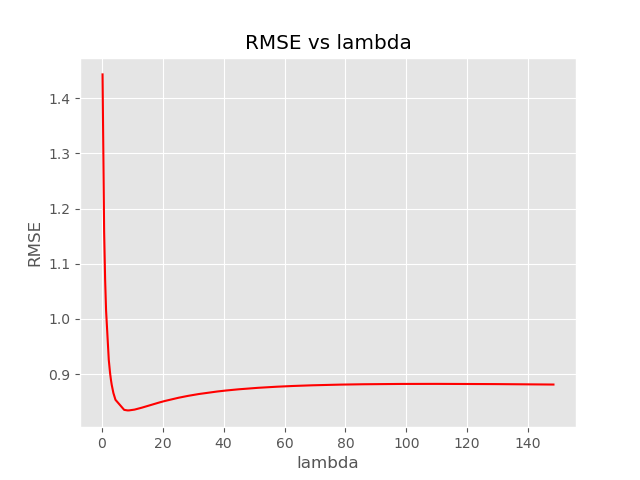
\includegraphics[scale=0.5]{RMSE_vs_lambda.png}
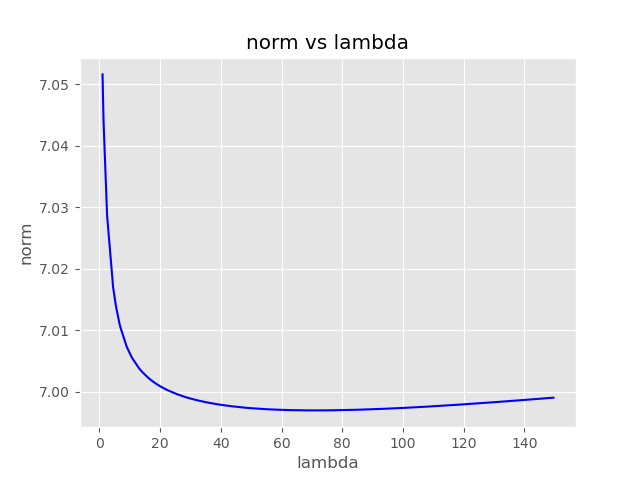
\includegraphics[scale=0.5]{norm_vs_lambda.png}

The optimal regularization parameter is  8.3910.\\
The RMSE on the validation set with the optimal regularization parameter is  0.8340.\\
The RMSE on the test set with the optimal regularization parameter is  0.8628.
\newpage
Part d:
To solve for the closed form solution, we first expand the objective function as the following:
\begin{align*}
	f &= \| Ax + b1 - y \|_2^2 + \| \Gamma x \|_2^2\\
&= (Ax + b1 - y)^T (Ax + b1 - y) + (\Gamma x)^T (\Gamma x)\\
&= (x^T A^T + b1^T - y^T) (Ax + b1 - y) + x^T \Gamma^T \Gamma x\\
&= x^T A^T Ax + 2b1^T Ax - 2y^T Ax - 2b1^T y + b1^2n + y^T y + x^T \Gamma^T \Gamma x
\end{align*}
Then, we can find the gradient of \( f \) with respect to \( x \) and \( b \).\[
\nabla_x f = 2A^T Ax + 2bA^T 1 - 2A^T y + 2\Gamma^T \Gamma x
\]

\[
\nabla_b f = 2 1^T Ax - 2 1^T y + 2bn 
\]

Next, we set $\nabla_b f = 0$ and solve for $b^*$, which results in
\[
b^* = \frac{1^T (y - Ax)}{n}
\]
Now, we can plug \( b^* \) back to the gradient with respect to $x$ and set it equal to $0$ solve for \( x^* \).
\begin{align*}
	(A^T A + \Gamma^T \Gamma)x + \left( \frac{1^T (y - Ax)}{n} \right) A^T 1 - A^T y &= 0\\
(A^T A + \Gamma^T \Gamma)x + \frac{1}{n} A^T 11^T y - \frac{1}{n} A^T 11^T Ax - A^T y &= 0\\
\left[ A^T A + \Gamma^T \Gamma - \frac{1}{n} A^T 11^T A \right] x &= A^T y - \frac{1}{n} A^T 11^T y\\
\left[ A^T \left( I - \frac{1}{n} 11^T \right) A + \Gamma^T \Gamma \right] x &= A^T \left( I - \frac{1}{n} 11^T \right) y\\
\end{align*}
Thus, $x^* = \left[ A^T \left( I - \frac{1}{n} 11^T \right) A + \Gamma^T \Gamma \right]^{-1} A^T \left( I - \frac{1}{n} 11^T \right) y$.
where \( I \) is the identity matrix and \( 1 \) is the one vector.

Then, we can calculate results using the closed form solution and find the difference between results from part c.

Difference in bias is  2.3657E-11\\
Difference in weights is  3.1597E-11

We can see that the differences are so small that they are negligible.

\newpage
Part e:

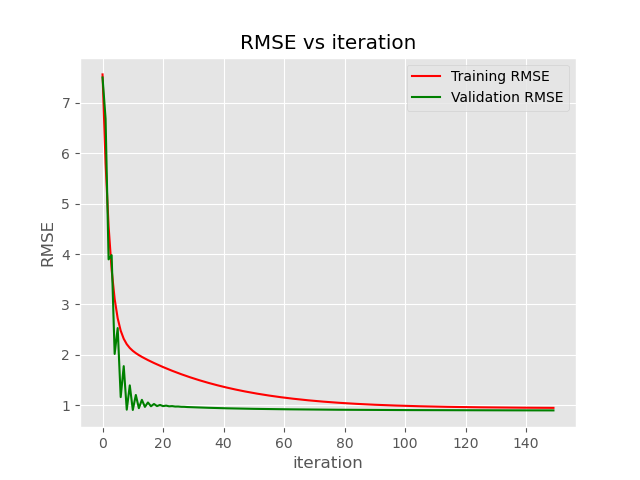
\includegraphics{convergence.png}

Difference in bias is  1.5388E-01\\
Difference in weights is  8.0269E-01
\end{solution}
\newpage

\end{document}
